
No caso monofásico, o retificador de meia onda associa somente um diodo na saída de tensão da fonte. Dessa forma, somente em um dos semiciclos (geralmente o positivo) da tensão alternada de alimentação $v\left( \omega t \right) $ há passagem de corrente para a carga.

No caso de uma carga resistiva pura, a estrutura do retificador monofásico de meia onda pode ser visto na figura \ref{fig:RMMOCR}.

\begin{figure}[h]
\center
\includegraphics[scale=0.55]{imagens/RetifMeiaOndaCargaResistiva.png}
\caption{Retificador monofásico de meia onda com carga resistiva.}
\label{fig:RMMOCR}
\end{figure}

Como mencionado acima, o diodo bloqueia o semiciclo negativo da tensão alternada, portanto a tensão aparente para a carga $R$ consiste somente dos semiciclos positivos.

Sendo a tensão de alimentação \[
v(\omega t)=\sqrt{2}V_o\sin(\omega t) 
\] podemos calcular a tensão média na carga
\begin{align*}
    V_{L,med} &= \frac{1}{2\pi}\int_\alpha^{\pi}\sqrt{2}V_o\sin(\omega t)d(\omega t) \\
	     &= \frac{\sqrt{2}V_o}{2\pi}[-\cos(\omega t)]_\alpha^{\pi} \\
	     &\approx 0,45 V_o
.\end{align*}

A corrente média na carga, então, é
\begin{align*}
    I_{L,med} &= \frac{1}{2\pi}\int_\alpha^{\pi}\frac{\sqrt{2}V_o}{R}\sin(\omega t)d(\omega t) \\
    &= \frac{V_{L,med}}{R} \\
    &\approx \frac{0,45 }{R}V_o
.\end{align*}


A corrente de pico no diodo $I_{D,p}$ é tal qual a corrente de pico na carga, ou seja, \[
I_{D,p} = \frac{\sqrt{2}V_o}{R}
,\] enquanto a tensão de pico inversa do diodo é \[
    V_{D,p} = \sqrt{2}V_o
.\] 

Para o dimensionamento correto do diodo é necessário saber o valor eficaz da corrente que passa por ele, ou seja,
\begin{align*}
    I_{L, ef} &= \sqrt{\frac{1}{2\pi} \int_{\alpha}^{\pi}\left(  \frac{\sqrt{2}V_o}{R}\right) ^{2}\sin^{2}(\omega t)d(\omega t)} \\
&=\sqrt{\frac{V_o^{2}}{\pi R^{2}}\int_{\alpha}^{\pi}\sin^2(\omega t)d(\omega t)} \\
&= \frac{V_o}{\sqrt{2}R} \approx 0.707\frac{V_o}{R}
.\end{align*}

No caso de uma carga RL com componente indutivo, a estrutura do retificador monofásico de meia onda pode ser vista na figura \ref{fig:RMMOACRL}.

\begin{figure}[h]
\center
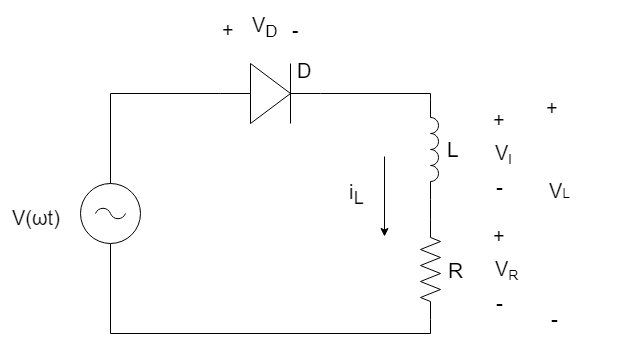
\includegraphics[scale=0.55]{imagens/cargaRl.png}
\caption{Retificador monofásico de meia onda com carga com componente indutivo}\label{fig:RMMOACRL}
\end{figure}

Agora, devido à indutância, há uma defasagem entre a corrente e a tensão, então o diodo não mais impede a passagem de corrente quando $\omega t = \pi$, mas em um ângulo $\beta$ maior do que $\pi$, como observado na figura \ref{fig:FO}. Ou seja, enquanto a corrente não se anula, o diodo continua conduzindo e, portanto, a tensão na carga torna-se negativa para ângulos superiores a $\pi$.

\begin{figure}[h]
\center
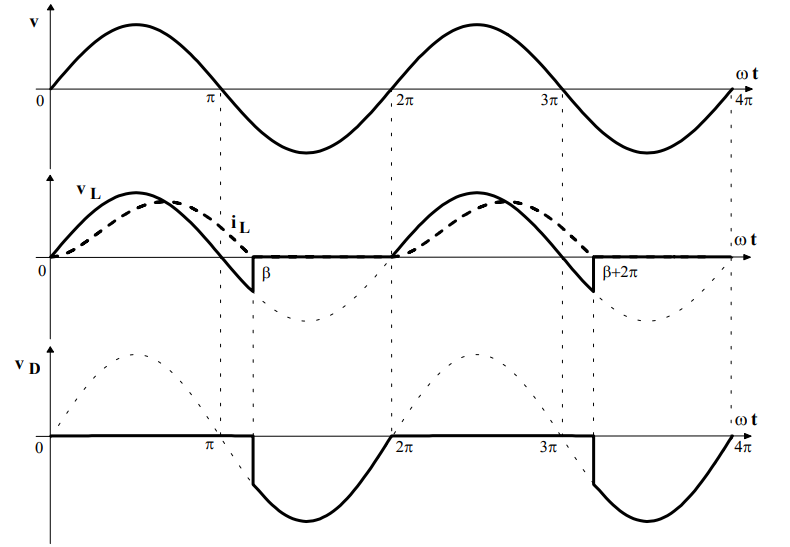
\includegraphics[width=0.6\textwidth]{imagens/FormasOndas.png}
\caption{Formas de onda das tensões e corrente no circuito do retificador de meia onda a diodo com carga indutiva.}\label{fig:FO}
\caption*{Fonte: EI I - Capitulo 2 - UNESP \protect\footnotemark}
\end{figure}

\footnotetext{Disponível em: <www2.sorocaba.unesp.br/professor/flavioasg/ei/cap2.pdf> Acesso em set. 2018.}

Nesse circuito, modelamos a corrente na carga $I_L$ pela equação \[
I_{L}(\omega{t}) = {\frac{\sqrt{2}V_o}{\sqrt{R^2 + X^2}}\sin{\left(\omega{t}-\phi\right)} - I_{1}\left(0\right)e^{-t/\tau}}
,\] onde $\phi = \arctan{\frac{X}{R}}$, $ {X} = \omega{L} $,  $\tau = \frac{L}{R}$.

Podemos dividir a corrente do circuito em dois componentes $I_L = i_1 + i_2$, de forma que
\begin{align*}
    i_{1}(\omega{t}) &= {\frac{\sqrt{2}V_o}{\sqrt{R^2 + X^2}}\sin{\left(\omega{t}-\phi\right)}}\\
	i_{2} &= I_{1}\left(0\right)e^{-t/\tau}
\end{align*}
A corrente $i_{2}$ pode ser entendida como a corrente do transitório, enquanto $i_{1}$ é a resposta em regime permanente da carga RL, conforme ilustrado na figura \ref{RMMOACRLI}.

Sabendo que $I_{1}(0) = {\frac{\sqrt{2}V_o}{\sqrt{R^2 + X^2}}}\sin{(-\phi)}$, obtêm-se a expressão \[
 I_{L}(\omega{t}) = {\frac{\sqrt{2}V_o}{\sqrt{R^2 + X^2}}[\sin{\left(\omega{t}-\phi\right)} - \sin{(-\phi)}e^{-t/\tau}}]
.\]

\begin{figure}[h]
\center
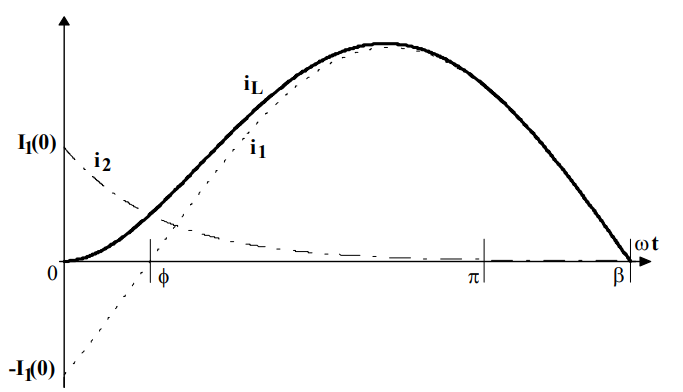
\includegraphics[width=0.6\textwidth]{imagens/correntedecarga.png}
\caption{Corrente de carga como no circuito da figura \ref{fig:RMMOACRL}.}\label{RMMOACRLI}
\caption*{Fonte: EI I - Capitulo 2 - UNESP $^1$}
\end{figure}

Quanto à tensão média aplicada na carga, é necessário modelar o valor do ângulo $\beta$. Para tal, observa-se que $i_{\omega}{t} = 0 $ quando ${\omega}{t} = {\beta}$.Dessa forma, substituindo ${\omega}{t} = {\beta}$ e sabendo que ${\omega}{\tau} = {\frac{\omega{L}}{R}} = {tg}{(\phi)}$, \[
\sin({\beta}-{\phi}) + \sin({\phi}){e^{-\beta/{ \tan({\tau})}}} = 0
.\] A relação entre $\beta$ e $\phi$ pode ser observada na figura \ref{fig:ACFA}. Portanto,
\begin{align*}
    V_{L,med} &= {\frac{1}{2\pi}{\int_{0}^{\beta}\sqrt{2}{V_o}{\sin({\omega}{t})}}d({\omega}{t})} \\
&\approx 0,225{V_o(1 - \cos({\beta}))}
.\end{align*}

\newpage
\begin{figure}[ht]
\center
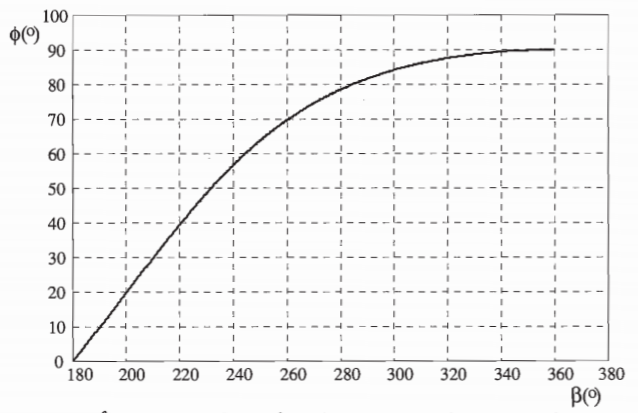
\includegraphics[scale=0.8]{imagens/grafico_variacao_beta_com_phi.PNG}
\caption{${\beta}$ em função de ${\phi}$.}\label{fig:ACFA}
\caption*{Fonte: Eletrônica de Potência (2006)}
\end{figure}

A partir dessa equação, vê-se que a tensão média na carga é inferior ao caso puramente resistivo. Além disso, como $V_{L,med} = 0 $ \[
I_{L,med} = \frac{0,225{V_o(1 - \cos({\beta}))}}{R}
.\] 

Uma forma de combater os efeitos da indutância no circuito é através de um diodo roda livre paralelo à carga. Dessa forma o circuito apresenta duas etapas de funcionamento. A primeira durante o semiciclo positivo da tensão de alimentação, na qual o diodo principal encontra-se polarizado e o diodo de roda livre está polarizado reversamente. A segunda durante o semiciclo negativo, na qual a corrente resultante da ação da indutância circula pelo diodo de roda livre, polarizado diretamente, enquanto o diodo principal polariza-se inversamente. A resposta desse circuito pode ser analisada através da figura \ref{fig:VIDRL}.

\begin{figure}[ht]
\center
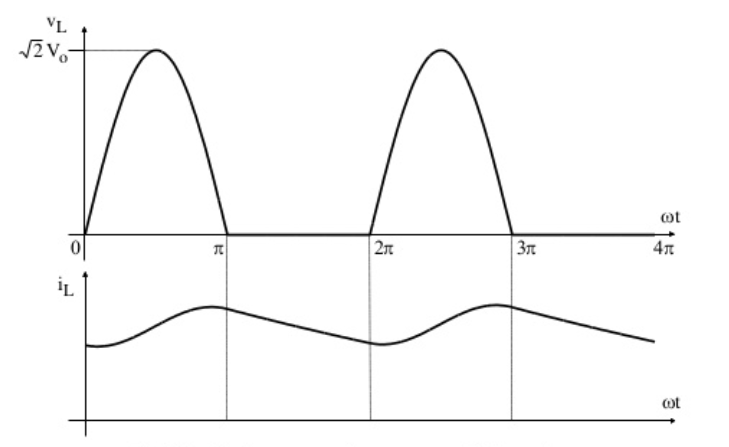
\includegraphics[scale=0.75]{imagens/VeIparaDRL.PNG}
\caption{Tensão e corrente na carga com componente indutivo no circuito com diodo de roda livre para condução contínua.}\label{fig:VIDRL}
\caption*{Fonte: Eletrônica de Potência (2006)}
\end{figure}

Para obter o modelo da corrente e da tensão na carga supõe-se que a estrutura encontra-se em regime permanente e em condução contínua. Pela série de Fourier para o sinal de entrada senoidal, podemos escrever \[
V_{L}(\omega{t}) = \frac{\sqrt{2}V_o}{\pi} + \frac{\sqrt{2}V_o}{2}{\sin({\omega}{t})} - {2}\frac{\sqrt{2}V_o}{\pi}[{\frac{\cos(2{\omega}{t)}}{1\cdot 3}}+{\frac{\cos(4{\omega}{t)}}{3\cdot 5}}+{\frac{\cos(6{\omega}{t)}}{5\cdot 7}}...] 
,\] ou seja, a tensão e a corrente médias na carga serão 
\begin{align*}
    V_{L,med} &= 0,45 V_o \\
    I_{L,med} &= \frac{0,45_o}{R}
.\end{align*}

Uma situação comum do uso do retificador é quando é alimentado por um transformador, que permite a adaptação da tensão da fonte à tensão de operação da carga e o isolamento entre a carga e a rede. O circuito nessa situação torna-se o da figura \ref{fig:TD}.

\begin{figure}[ht]
\center
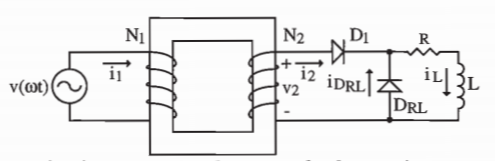
\includegraphics[scale=0.9]{imagens/trasformador_diodo.PNG}
\caption{Retificador monofásico de meia onda com diodo roda livre alimentado por um transformador.}\label{fig:TD}
\caption*{Fonte: Eletrônica de Potência (2006)}
\end{figure}

A figura \ref{fig:FdOTD} ilustra as formas de ondas para o circuito apresentado acima.

\begin{figure}[ht]
\center
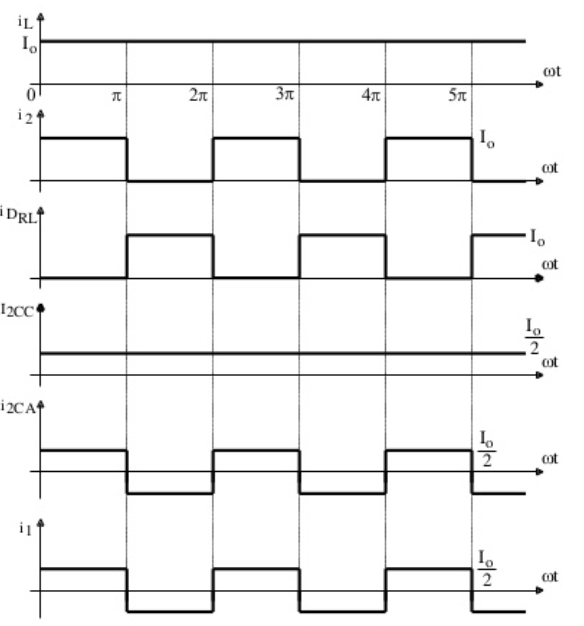
\includegraphics[scale=0.9]{imagens/formasdeOndaTransformador.PNG}
\caption{Formas de onda para o circuito da figura \ref{fig:TD}.}\label{fig:FdOTD}
\caption*{Fonte: Eletrônica de Potência (2006)}
\end{figure}

Sabemos que a potência e a tensão média da carga são dadas por
\begin{align*}
    P_{L} &= V_{L,med}\cdot I_{L,med} \\
    V_{L,med} &= 0,45 V_2
.\end{align*}

O uso mais comum para o retificador monofásico de meia onda é na alimentação da armadura de pequenos motores de corrente contínua, na alimentação de enrolamentos de excitação de máquinas elétricas, no carregamento de baterias e na alimentação de circuitos eletrônicos. 

